% 英文で執筆する場合はクラスファイルへのオプションを[T,E]としてください.
% If you want to write your paper in English, pass to [T,E] options to document class.
\documentclass[T,J]{fose} % 「コンピュータソフトウェア」用のクラスファイルは compsoft です.
\taikai{2024} % 固定です.出版委員長が毎年変更してAuthor Kitを配布してください.

\usepackage[dvipdfmx]{graphicx}
\usepackage{xcolor} % 色を扱うためのパッケージ

% ユーザが定義したマクロなどはここに置く.ただし学会誌のスタイルの
% 再定義は原則として避けること.

% 以下のマクロはサンプルファイル作成用のマクロです.不要であれば削除してください.
\newcommand{\todo}[1]{\colorbox{yellow}{{\bf TODO}:}{\color{red} {\textbf{[#1]}}}}
\newcommand{\change}[1]{\colorbox{green}{{\bf CHANGE}:}{\color{black} {\textbf{[#1]}}}}
\newcommand{\rqone}{開発者とパターンに関係性はあるのか}
\newcommand{\rqtwo}{パターンマッチによって収集されたパターンの信頼度はどの程度か}

% 以下は説明のために使用したパッケージであるため,削除可能.
\usepackage{listings}
\usepackage{tabularx}
\usepackage{fancyvrb}
\usepackage{xurl}
\usepackage{cite}


\usepackage{subcaption}
\begin{document}

% 論文のタイトル
\title{複数のプロジェクト間で共通して頻繁に修正されるソースコード改善内容の分析}
% 以下の \etitle(と\@etitle)はFOSE論文フォーマット独自のマクロです.
% FOSEに投稿した論文を発展させてコンピュータソフトウェアに投稿される場合はコメントアウトしてください.
% \setetitleは奇数ページのヘッダに表示する文字列(\etitle)を設定するためのマクロです.
% タイトルが2行に渡る場合は "\\" を 使用することで任意の位置で改行をすることができます.
\setetitle{Analysis of Common Prevalent Code Improvements between Multiple Projects}
%\setetitle{Long Long Long Long Long Long \\ Long Long Long Long Long \\ Long Long Long Long Long Long Long Long Long Long Long Long Paper Title}

% タイトル,著者などが複数行にわたり,論文冒頭の著者名が日本語アブストと重複して描画された場合に以下のコメントアウトを外してください.
%\longtitle

% 著者
% 和文論文の場合,姓と名の間には半角スペースを入れ,
% 複数の著者の間は全角スペースで区切る
%
\author{野口 朋弥 伊原 彰紀}
%
% ここにタイトル英訳 (英文の場合は和訳) を書く.
% 英語タイトルは論文1ページ目左下,著者らの名前・所属一覧の一番上に表示される
%
% 上記\setetitle中で改行した場合は "\etitle" を削除し,改行(\\)を入れていないタイトルを記載してください.
% \ejtitleは1ページ目左下に挿入されるタイトルとして使用されます.
% また,"\etitle"はFOSE論文フォーマット独自のマクロです.
\ejtitle{Analysis of Common Prevalent Code Improvements between Multiple Projects}
%
% ここに著者英文表記 および
% 所属 (和文および英文) を書く.
% 複数著者の所属はまとめてよい.
%
\shozoku{Tomoya Noguchi, Akinori Ihara}{和歌山大学}
{Wakayama University}
}

%
% 和文アブストラクト
% In English paper, content of Jabstract will be ignored. 
\Jabstract{ソフトウェア開発では, ソースコードの保守性や品質を維持するためにコーディング規約を用いてコーディングスタイルを統一する. しかし, コーディング規約には含まれない規則も存在し, このような規則は静的解析ツールで検出することが容易でない. 従来研究では, 過去の開発履歴から頻出する修正パターンを収集する手法を開発しているが, パターンを収集するためには十分な開発履歴を要する. 本研究では, 異なるプロジェクト間で頻繁に修正されるソースコードの改善内容を分析する.\todo{繋がりがない}ケーススタディとして\todo{XX}を分析した結果\todo{hoge}}


\maketitle \thispagestyle {empty}
%%%%%%%%%%%%%%%%%%%%%%%%%%%
\section{はじめに}
%%%%%%%%%%%%%%%%%%%%%%%%%%%

ソフトウェア開発では,保守が容易になるソースコードを作成することが将来の改修コストを下げることとなる\cite{costdown}.特にオープンソースソフトウェアのような複数人で開発を行う組織では,様々なコーディングスタイルで実装するため,開発者らに命名規則や禁止事項などを規定されたコーディング規約を周知し,コーディングスタイルを統一している\cite{EffectsSAT}.しかし,コーディング規約には具体的な記述がないコーディングスタイルの問題が存在する.\cite{ueda2020}
%ソースコードにおけるコーディング規約に違反している箇所を機械的に特定するために静的解析ツールが使用される.静的解析ツールは,ソースコード中に含まれるコーディング規約に違反している箇所や,コードの複雑度や可読性の評価,バグ検出など多岐にわたる機能を提供している.そのため,開発者は静的解析ツールを使用することで,ソースコードの保守性や可読性を向上させることができる.しかし,静的解析ツールでは,検出できないソースコードも存在し,
特に実行エラーが発生することのない言語特有の記法は,コーディング規約に具体的な記述がないことが多く,記法に慣れていない開発者は非イディオマティックなソースコードを実装する\cite{idiom}.その結果,コーディングスタイルにそぐわないソースコードの変更提案は,コードレビューを通して修正される.


% コードレビューには多大な時間がかかるため,ソースコード自動修正をはじめとする多くの研究が進められている\cite{reviewcost}\cite{reviewcost2}\cite{Automatingcodereview}\cite{towardsImproving}\change{参考文献追加}\todo{もっと書く}.
Uedaらは,プロジェクトが周知するコーディング規約に含まれないが,頻繁に修正されるコーディングスタイルを検出するためのツールDevReplayを開発している.\cite{devreplay}当該手法は,開発履歴から頻出するソースコードの修正方法をトークン単位でパターンとして収集しておき,頻繁にコードレビューで指摘を受けるソースコードの修正案を開発者に提示する.DevreplayをOSSの実プロジェクトに適用することでコードレビューのコストを削減可能なことを明らかにしている.しかし,従来手法では過去の開発履歴が少ない場合,パターンを十分に収集できず,ソースコード修正の精度が低下する可能性がある.

% 静的解析ツールによって特定できなかったパッチ作成者が作成したプロジェクトのコーディングスタイルにそぐわないソースコードの変更提案は,コーディレビューを通して修正が行われる.コードレビューではソースコードの検証,フィードバック,修正が行われる.しかし,コードレビューはソースコードの変更提案を検証するのに,多大な時間がかかる.\cite{reviewcost}\cite{reviewcost2}そのため,コーディングスタイルにそぐわないパッチを作成する開発者が増加すると,レビュワーが同じ指摘を複数行う必要があるため,コストがかかる.

% 従来研究では,プロジェクトのコーディングスタイルにそぐわないパッチを自動的に修正するために,過去の開発履歴から頻出するソースコードの修正方法をパターンとして収集し,事前にパッチに適用することで,コーディレビューのコストを削減する手法が提案されている.\cite{devreplay}従来研究では,収集されたパターンはコーディング規約に存在しない明示されていないパターンも存在し,実際のプロジェクトにおいても有用であることがわかっている.しかし,従来手法では過去の開発履歴が少ない場合,パターンを十分に収集できず,コードの修正を行うことができない.

本研究では,開発履歴が少ない場合に,複数のソフトウェア開発プロジェクトの開発履歴を統合をすることによって,十分なパターンを獲得する手法を提案する.具体的には,共通の開発者が多数参画するプロジェクトの開発履歴を統合することにより,パターンの獲得を期待する.ただし,共通の開発者の参画が少ないと,偽陽性(異なるコーディングスタイルのパターン)が増加し,有用なパターンを獲得できないことが示唆される.
%学習データ数を増やす手法を提案する.さらに,開発者を活動量を考慮したプロジェクトの統合をすることによる学習データの増強の効果についても分析する.
本研究では,コーディングスタイルに関する記述が充実しているNumPy組織\footnote{\url{https://github.com/numpy}}を対象に分析を行う.

まず初めに,共通の開発者が多数参画するプロジェクトの開発履歴を統合することで,共通の実装パターンを多数獲得できるか否かを調査する.ケーススタディとしてPython言語の数値計算ライブラリを構成する21プロジェクト\todo{分析したのは2,対象は21}を対象に調査する.

%RQ1では,パターンの増強をするのに,開発者が類似しているプロジェクトのパターンを流用することが有用かを確かめるために,参加する開発者が類似するプロジェクトは,生成されたパターンも類似しているのかを確かめるために,開発者が1番多く参加しているnumpyと,開発者が10人以上で類似度が0ではなかったnumpy-refactor,numpydoc,numpy-financialの3つのプロジェクトを対象にパターンの類似度を調査する.

次に,パターンの信頼度を測定することで,プロジェクトにおいて有用なパターンを生成できているかを調査する.対象プロジェクトのコミット開始から10年のデータを対象に,\ref{sec:method}章の手法でパターンを生成,フィルタリングを行うことで,プロジェクトにとって有用なパターンを特定する.
% \noindent\textbf{RQ2: \rqtwo}
% \todo{ここよくわからんので直せない}RQ2では, RQ1で対象にしたペアにおいて,単体で\ref{subsubsec:filtering}の手法でパターンのフィルタリングを行った場合,ペアのプロジェクトのパターンを統合して,フィルタリングを行った時に,信頼度のあるパターンの総数に変化があるのかを調査する.

以降,\ref{sec:union}章でソフトウェア開発におけるコーディングスタイルの重要性と,従来研究について述べる.その後,\ref{sec:method}章で本研究におけるパターンの収集方法と,パターンのフィルタリング方法について述べる.\ref{sec:casestudy}章,\ref{sec:discussion}章でケーススタディで行った結果と考察について述べ,\ref{sec:conclusion}章でまとめる.

%%%%%%%%%%%%%%%%%%%%%%%%%%%
%2章背景
\section{コーディングスタイルの統一}\label{sec:union}
%%%%%%%%%%%%%%%%%%%%%%%%%%%

\subsection{コーディングスタイル}
コーディングスタイルは,ソースコードの記述方法や構造に関する記法を指す.ソフトウェア開発では,コーディングスタイルを統一させるためのコーディング規約を開発者に周知し,規約に準拠したソースコードを開発することで保守性や可読性を向上させている.\cite{AnalysisoftheTools}コーディング規約は,プログラムにおける命名規則,禁止事項などを規定したルールである.コーディング規約は各プログラミング言語で存在し,Python言語のPEP8,Java言語のCode Conventions for the Java Programming Languageが一般的である.これらのコーディング規約はそれぞれ多少の違いがあり,Java言語のCode Conventions for the Java Programming Languageではインデントにタブかスペースを使用することが許容されているが,Python言語のPEP8ではインデントにはスペースを使用することが推奨されており,タブは使用しないように推奨されている.

% コーディングスタイルは,ソフトウェア開発において,ソースコードの記述方法や構造に関する一連のガイドラインやルールを示す.コーディングスタイルを統一させるために,コーディング規約などを使用することで,保守性や可読性を向上させている.
% コーディング規約とは,プログラムにおける規則について定められており,命名規則,禁止事項などを規定したルールのことである.コーディング規約はプログラミング言語ごとに複数存在し,具体的にはPython言語のPEP8,Java言語のCode Conventions for the Java Programming Languageのようにプログラミング言語ごとに定められている.しかし,これらのコーディング規約は規約ごとに多少の違いがあり,具体的には,Java言語のCode Conventions for the Java Programming Languageではインデントにタブかスペースを使用することが許容されているが,Python言語のPEP8ではインデントにはスペースを使用することが推奨されており,タブは使用しないように推奨されている.

開発者がコーディング規約への違反を目視で検出するためには多くのコストを要するため,コーディング規約に違反している箇所を機械的に特定する静的解析ツールが使用される\cite{AnalysisoftheTools}.静的解析ツールも言語別に複数の種類があり,参照している規約の種類や,違反を検出した際のメッセージのフォーマットや,検出する違反のカスタマイズ性の高さなどが異なる.しかし,特に実行エラーが発生することのない言語特有の記法は,コーディング規約に具体的な記述がないことが多く,静的解析ツールで検出できない.例えば,Java言語やC言語で使用される繰り返しの構文を,Python言語ではリスト内包表記で記述することができ,これは言語特有の記法である.Python言語ではいずれの記法であっても実行エラーになることはない.記法に慣れていない開発者が実装する非イディオマティックでコーディングスタイルに準拠していないソースコードは,コードレビューによる指摘で修正されることが多い\cite{idiom}.


% 大量の違反の検出結果には修正する必要がないような軽微な違反も含まれ,それらを開発者がレビューし保守するには多くのコストを要するため困難である.
% さらに様々な違反から優先して修正すべき規約違反を特定することは,開発の経験や,複雑なソースコードの理解が必要であるため,プロジェクト開発において容易でない\todo{要引用}.
% %Brittany Johnson, Yoonki Song, Emerson Murphy-Hill, and Robert Bowdidge. Why don’t software developers use static analysis tools to find bugs? In Proceedings of the 35th International Conference on Software Engineering (ICSE’13), pp. 672–681, 2013


% ソースコードにおけるコーディング規約に違反している箇所を機械的に特定するために静的解析ツールが使用される.静的解析ツールは,ソースコード中に含まれるコーディング規約に違反している箇所や,コードの複雑度や可読性の評価,バグ検出など多岐にわたる機能を提供している.そのため,開発者は静的解析ツールを使用することで,ソースコードの保守性や可読性を向上させることができる.しかし,静的解析ツールでは,検出できないソースコードも存在し,具体的にはPython言語だけ存在するリスト内包表記などのイディオムはPython言語を主に使用している開発者しか知らず,Java言語などの他の言語を主に使用している開発者はこの記述方法を知らないため,非イディオマティックなコードを書いてしまう.\cite{idiom}\todo{この段落すべて前文で言ってる}

% パッチ作成者が導入したプロジェクトのコーディングスタイルにそぐわないソースコードの変更提案は,コードレビューを通して修正が行われる.しかし,コードレビューはソースコードの変更提案を検証するのに多大な時間がかかる.\cite{reviewcost}そのため,コーディングスタイルにそぐわないパッチを作成する開発者が増加すると,レビュワーが同じ指摘を複数行う必要があるため,コストがかかる.
\subsection{従来研究}
従来研究はコーディングスタイルに準拠していないパッチを自動修正するために,開発履歴で頻出するソースコードの修正方法をパターンとして収集しておき,頻繁にコードレビューで指摘を受けるソースコードの修正案を開発者に提示する手法が提案されている\cite{AutomaticPatch}\cite{findBugs}\cite{Relntancer}\cite{don'tDIY}

Uedaらは,プロジェクトが周知するコーディング規約に含まれないが,頻繁に修正されるコーディングスタイルを検出するためのツールDevReplayを開発している.当該手法は,開発履歴から頻出するソースコードの修正方法をトークン粒度でパターンとして収集しておき,頻繁にコードレビューで指摘を受けるソースコードの修正案を開発者に提示する\cite{devreplay}.\todo{1章と全く同じ文章}当該手法によって収集されたパターンでは,Pythonのコーディング規約には明示されていないパターンを獲得している.その他,ソースコード中のバグを修正するために,パターンマッチングを使用することで,ソースコードの修正が必要な箇所を特定する従来研究は数多くある\todo{もう少し具体的に書きたい}.

従来手法では,プロジェクトの開発初期では開発履歴が少なく,パターンを十分に収集できないためソースコード修正の精度が低下している.本研究では,開発履歴が少ない場合に,複数のソフトウェア開発プロジェクトの開発履歴を統合をすることによって,十分なパターンを獲得する手法を提案する.

% 本研究では開発履歴が少ないプロジェクトに対し,データの増強を目的としたプロジェクトの統合によりデータを増やす手法を提案する.この時,統合するプロジェクトは,プロジェクト固有のコーディングスタイルを損なわないようにするために,参加する開発者が類似しているプロジェクトを統合に用いる.

%%%%%%%%%%%%%%%%%%%%%%%%%%%
%3章アプローチ
\section{ソースコードの修正パターンの収集方法}\label{sec:method}
%%%%%%%%%%%%%%%%%%%%%%%%%%%

本研究では,従来研究で提案されたソースコードの修正パターンの収集方法を再現する(\ref{subsec:collect}節).その後,本研究では異なるプロジェクトから収集した修正パターンの統合方法を提案する(\ref{subsec:integrate}節).図\ref{fig:pattern_generate}は,本研究手法の概略図を示す.

%系列パターンマイニングとは,2つ以上のシーケンスから関連するパターンを見つけるためのよく知られている手法である.\cite{freespan}
% 系列パターンマイニングは,シーケンスデータセットから,頻度の高い要素の順序付きリストを抽出する.\cite{Miningcodingpattern}
%シーケンスデータセットは、ソースコードトークンなどの要素の順序付きリストを表すシーケンスで構成され、コードレビュープロセスにおける初期パッチと統合パッチの間の変更をキャプチャする。
%-------------------
\begin{figure*}[t]
\centerline{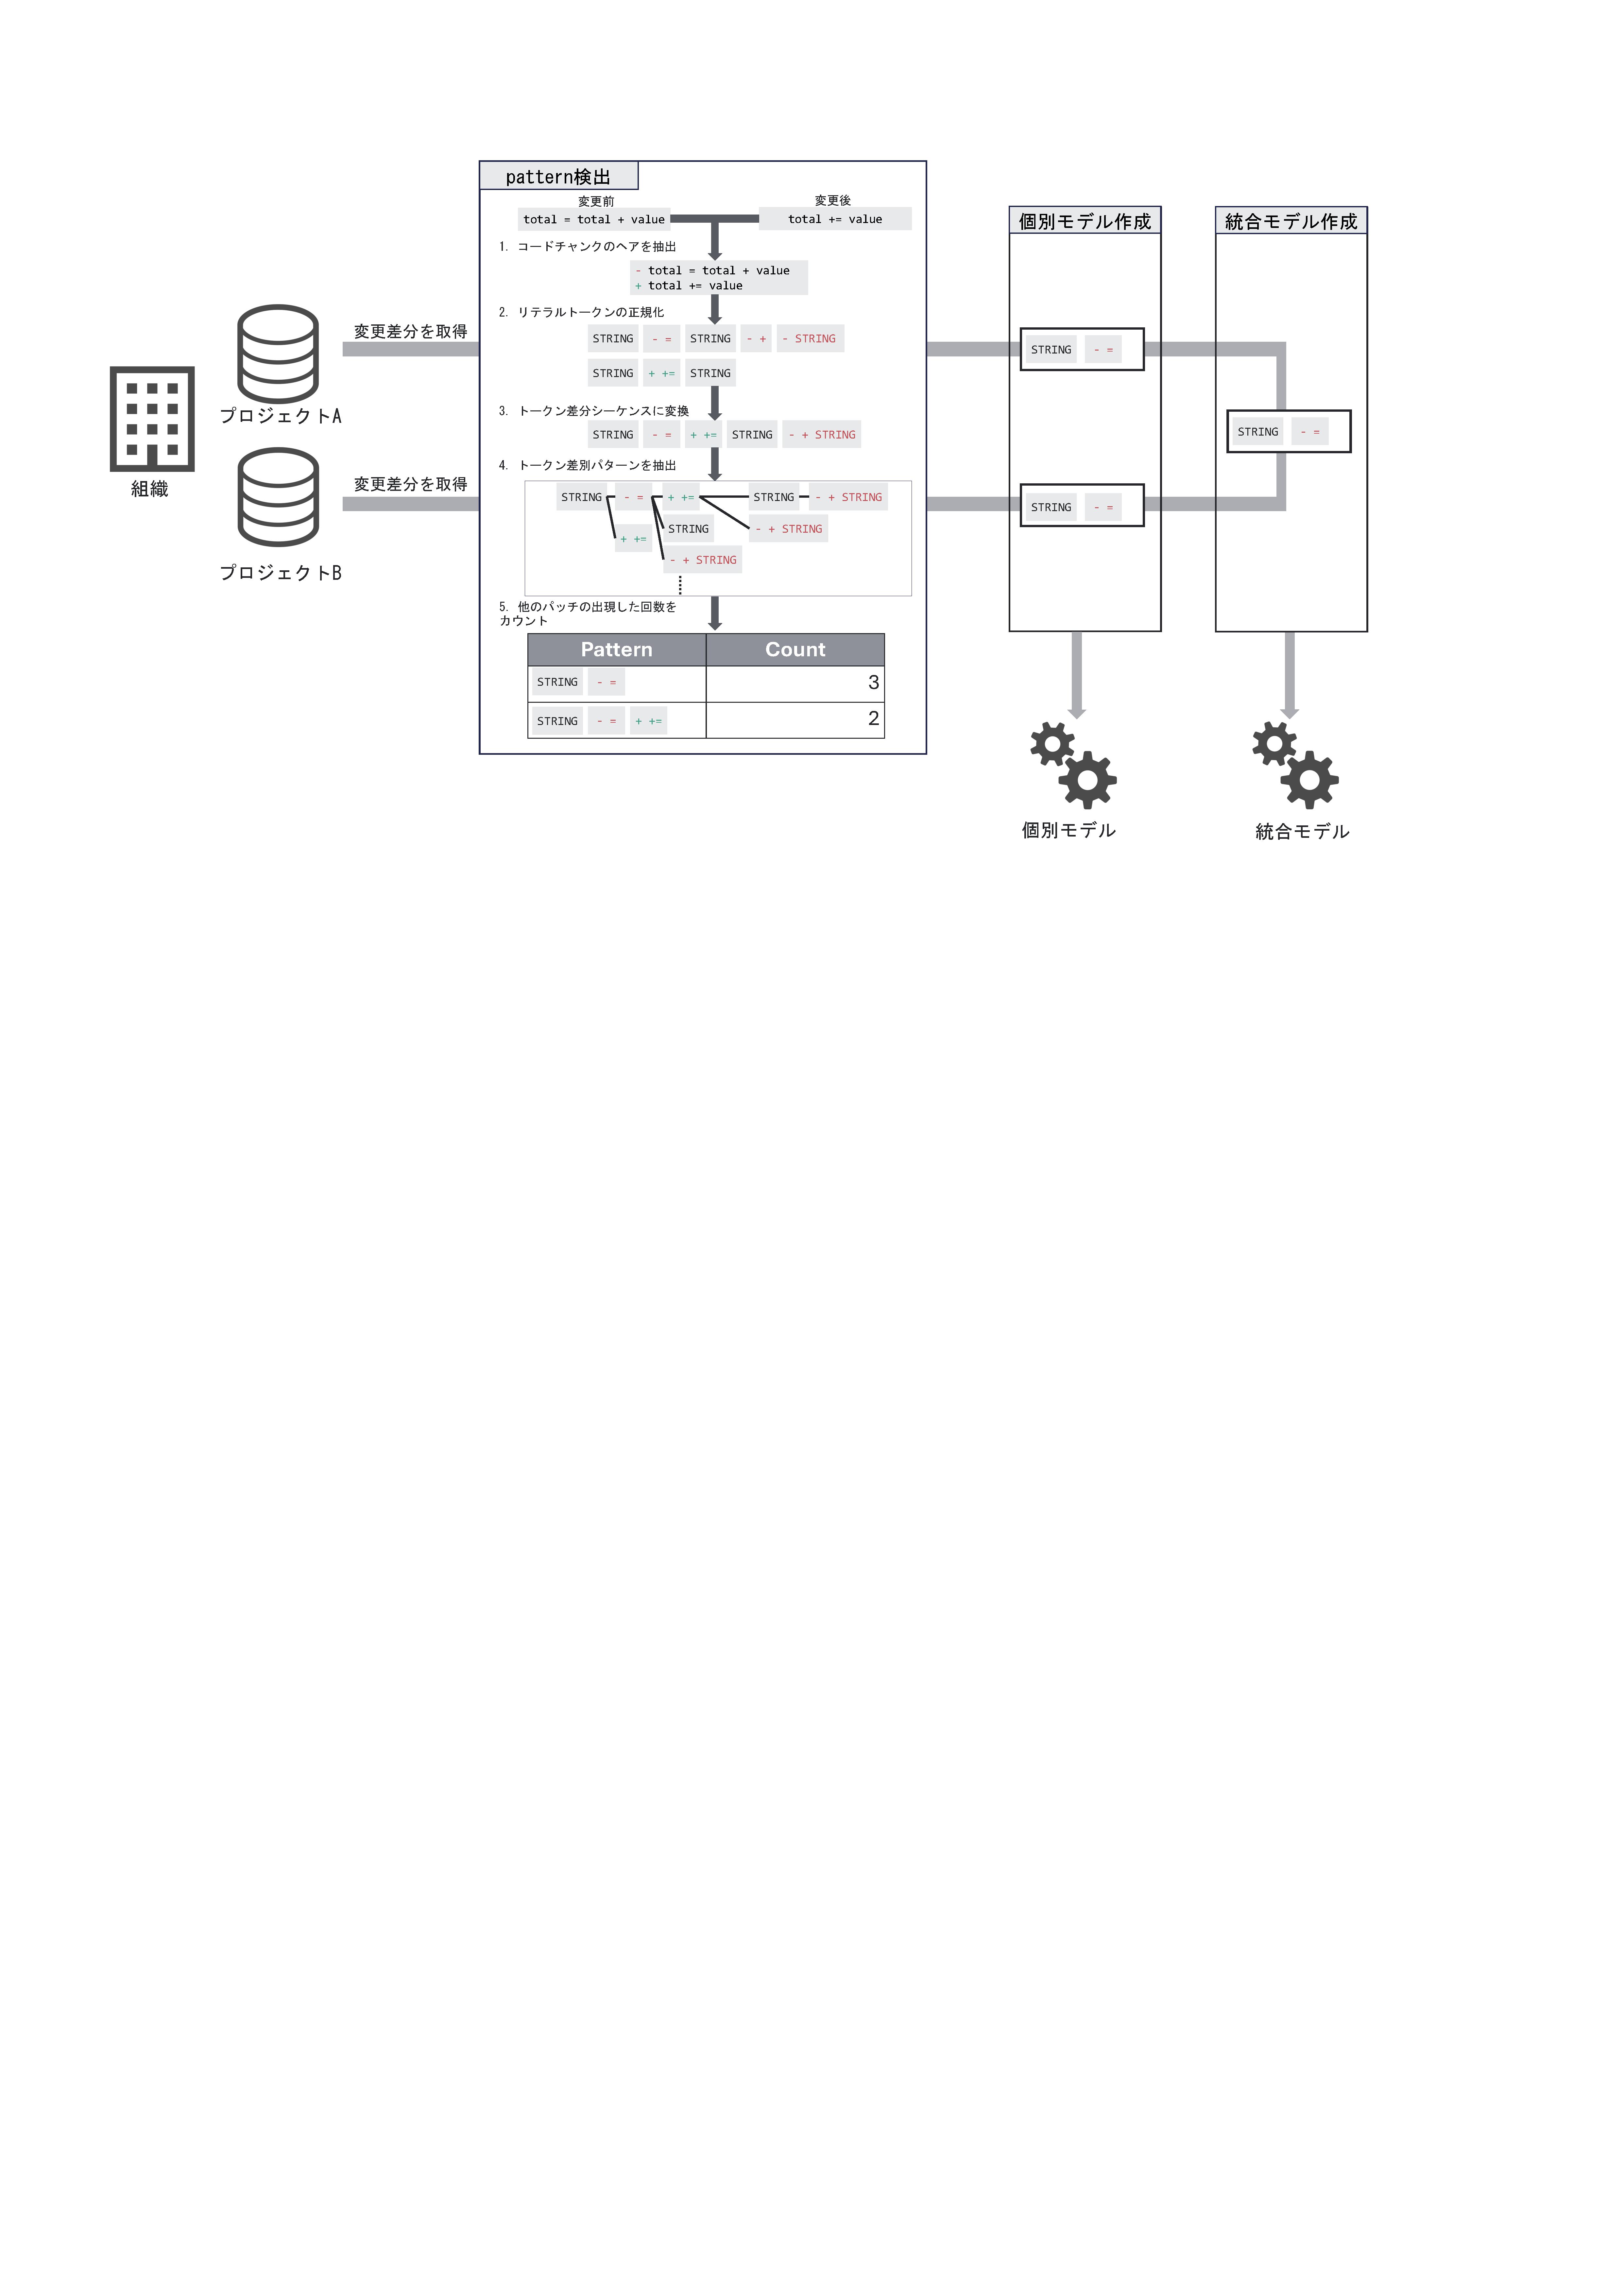
\includegraphics[width=1.0\linewidth]{Noguchi_fig/pattern_generate.pdf}}
\caption{研究手法の概略図}
\label{fig:pattern_generate}
\end{figure*}
%-------------------

\subsection{修正パターンの収集方法}\label{subsec:collect}
\subsubsection{パターン収集の手法}\label{subsubsec:collect_pattern}

パターンの生成には系列パターンマイニングを用いる.系列パターンマイニングは,2つ以上の連続するシーケンス(本研究ではトークン)からパターンを見つけるために用いられる手法である\cite{freespan}.具体的なパターンの収集は,次の5ステップで構成される.
\begin{enumerate}
    \item ソフトウェア開発プロジェクトのGitHubリポジトリに記録される分析対象区間の全てのコミットから,初期パッチと統合パッチを収集し,それぞれのパッチから抽象構文木(AST)を用いて変更されたコードチャンク(連続したソースコード行)を抽出する.
    %\item 初期パッチと統合パッチのペアからコードチャンク(連続したコード行)のペアを抽出する.このペアは,抽象構文木(AST)を用いて変更されたコードチャンクのみを抽出している.
    \item 汎用的な修正パターンを作成するために,数値リテラルは`\texttt{NUMBER}'に,図\ref{fig:pattern_generate}に示す文字リテラル`\texttt{total}'や`\texttt{value}'は`\texttt{STRING}'の文字列に正規化する.その後,抽象構文木でトークン単位の差分を抽出し,変更前のトークンと変更後のトークンを比較し,削除されたトークンの文頭には`\texttt{-}',追加されたトークンには`\texttt{+}'を先頭に付加する.\todo{並びが重要だから変数の正規化でIDは付与していない.}
    %\item 汎用的な修正パターンを作成するために,NUMBERリテラルとSTRINGリテラルのトークンを正規化する.図\ref{fig:pattern_generate}の例では,'total','value'といった文字列リテラルのトークンを'STRING'として扱っている.その後,トークン単位の差分をASTベースで算出し,変更前と変更後のトークンを比較し,削除されたトークンには'-',追加されたトークンには'+'を先頭に付加する.
    \item 系列パターンマイニングを実施する対象データセットとして,\todo{何がデータセット?}行の差分をトークンの差分シーケンスに変換する.前の手順でトークンが連続して`\texttt{-}',`\texttt{+}',または何も付加されていないトークンが連続した時は,連続したトークンを1つのトークンとして扱う.
    具体的には,手順2で正規化したトークン列の1行目に含まれる\colorbox{lightgray}{\texttt{- +}} \colorbox{lightgray}{\texttt{- STRING}}の2つのトークンは連続して文頭に`\texttt{-}'が付加されている.このようなトークン列は\colorbox{lightgray}{\texttt{- + STRING}}という1つのトークンとして扱う.\change{具体例の説明変更}\todo{意味不明}
    % 具体的には,'- +'のトークンと'- STRING'のトークンでは連続して'-'が付加されているため,'- + STRING'として扱う.\todo{この具体的...よくわからん}
    \item 系列パターンマイニングにより,トークン差列パターンを抽出する.具体的には,効率的な系列パターンマイニングの1つであるPrefixspanアルゴリズムを使用する\cite{prefixspan}.図\ref{fig:pattern_generate}では,`\texttt{STRING}'から始まる全てのトークンの組み合わせをパターンとして生成する.
    \item 分析対象期間で収集した全てのパターンの出現頻度をカウントする.
\end{enumerate}



\subsubsection{パターンのフィルタリング}\label{subsubsec:filtering}
分析対象データセットから生成した修正パターンの中には,冗長なパターンが含まれる.本研究では,4つのフィルタリングアプローチで\todo{によって}冗長なパターンを削除する.\todo{4つなのに箇条書き3つ}
\begin{itemize}
    \item 変更を示唆しない(追加または削除のみ)パターンを除去する.具体的には,(\colorbox{lightgray}{\texttt{STRING}} \colorbox{lightgray}{\texttt{- =}})のようなパターンを削除する
    \item 重複するパターンを除去する.具体的には,(\colorbox{lightgray}{\texttt{STRING}} \colorbox{lightgray}{\texttt{- =}} \colorbox{lightgray}{\texttt{+ +=}})は(\colorbox{lightgray}{\texttt{STRING}} \colorbox{lightgray}{\texttt{-=}} \colorbox{lightgray}{\texttt{+ +=}} \colorbox{lightgray}{\texttt{STRING}})
    
    具体的には,(`\texttt{STRING}' `\texttt{- =}' `\texttt{+ +=}')は(`\texttt{STRING}' `\texttt{-=}' `\texttt{+ +=}' `\texttt{STRING}')の一部とみなせるため,前者のパターンを削除する.
    \item データセット全てにおいて,提案手法を適用後,1度しか出現していないパターンを削除する.
\end{itemize}

最後に,各パターンの出現頻度をパターンの信頼度と捉え,式\ref{eq:confidence}で信頼度を算出する.本研究では従来研究と同様に信頼度10\%以下のパターンを削除する.

\begin{equation}\label{eq:confidence}
\text{信頼度} = \frac{\text{パターンによって正しく変更されたパッチ数}}{\text{パターンによって検出可能なパッチ数}}
\end{equation}\todo{正しく変更されたパッチとは?}
        % トリガー可能なパッチとは,パターンによって変更を行うことができるトークンを含んでいるパッチのことである.具体的には,('STRING' '- =' '+ +=')というパターンが存在した時に,このパターンを適用できるのは,('STRING' '=')というトークン列を持つパッチにおいて,このパターンを適用できる.一方,実際の変更後のパッチの数とは,パターンによって修正することが可能な変更後のパッチの数である.

\subsection{パターン数増強を目的としたプロジェクトの統合}\label{subsec:integrate}\todo{パターン数の}

\todo{RQ1が今まで出てないのにRQ2から始まってる}RQ2は,2つのソフトウェア開発プロジェクトの開発履歴を統合することによって修正パターンを増加を狙いとする.\todo{修正パターンの}本研究では,コーディングスタイルが類似するプロジェクトとして,2つのプロジェクト間で共通の開発者が参画し,それぞれのプロジェクトにおける活動量(コミット数)が類似しているプロジェクトのパターンを統合する.具体的には,2つのプロジェクトにおいて分析対象期間中にメインブランチにマージされたパッチ開発者を対象に,各開発者のコミット数をベクトル化し,両プロジェクトで作成したベクトルのコサイン類似度を用いてプロジェクト間の類似度を算出する.本研究では,プロジェクトのコーディングスタイルが,コミット数の多い開発者のスタイルに影響を受けていると考えたが,この仮説は確認できていない.プロジェクトと開発者のコーディングスタイルの違いの調査は今後の課題とする.

% ことによる,パターンを十分に生成できない問題に対処するため,他プロジェクトの開発履歴から生成されたパターンを用いた統合モデルを作成する.この時,プロジェクト固有のコーディングスタイルを反映するために,プロジェクトに参加している開発者に着目した手法を提案する,開発者を取得する手法として,プロジェクトに存在するログから,メインブランチにマージされたパッチの作成者を取得する.今回の手法では,対象期間内にパッチ作成者がコミットした数をベクトルとして扱い,開発者間の類似度を測定する.今回の手法では,コミット数しか反映しておらず,変更量は参照していないため,今後は変更量も考慮した開発者の類似を行う.

\textcolor{blue}{伊原ここまで確認済み}

%%%%%%%%%%%%%%%%%%%%%%%%%%%
%4章ケーススタディ
\section{ケーススタディ}\label{sec:casestudy}
%%%%%%%%%%%%%%%%%%%%%%%%%%%

\subsection{データセット}
Python言語の数値計算ライブラリ\todo{ん?}
本研究では,ソフトウェア開発プラットフォームであるGitHub上に存在するPython言語の数値計算ライブラリNumPy上の,Python言語で書かれたファイルが存在するプロジェクトを対象とした.\todo{ん?}プロジェクトの選定理由は,NumPyが充実したスタイルガイド\footnote{numpydoc v1.8.0rc3.dev0 Manual
: \url{https://numpydoc.readthedocs.io/en/latest/format.html}}を持っているため,スタイルガイドによる組織的なコーディングスタイルの統一性を評価することができると考えたからである.

本研究では,各分析対象プロジェクトにおいて,対象プロジェクトが最初にコミットした日から10年分のコミット履歴から存在するASTベースの置換によって検出可能な1行のコミットを分析対象とする.NumPyの21プロジェクト対象に分析を行う.データセットは,前半8割をパターンの生成用,後半2割をパターンの信頼度の評価のために用いる.

\subsection{分析手法}
参加する開発者が類似すると,生成されたパターンに類似しているのかを調査する,
プロジェクトに参加する開発者の類似度を以下のステップで算出した.
\begin{enumerate}
    \item 比較する2つのプロジェクト間で存在する全ての開発者の名前を取得
    \item ベクトルの次元を全ての開発者の数とし,ベクトルの要素を各プロジェクトにおいて開発者がコミットした数とする
    \item 算出したプロジェクトのベクトルをコサイン類似度を用いて比較
\end{enumerate}
この手法においてNumpyの組織に存在するプロジェクトでコサイン類似度を算出した時のヒートマップが図\ref{fig:dev_similarity}である.本研究では,コサイン類似度が\texttt{0.99}と一番高いnumpyとnumpy-refactorを\ref{subsubsec:collect_pattern}章の手法でパターンを生成する.

パターンの出現回数がパターンの類似度に影響を与えるのかを確認するために,パターンが出現した回数を意味するサポート値が2から20の範囲でパターンの一致度を図る.対象にしたパターンの一致度を計算した結果が図\ref{fig:num_numref_match}である.numpyのサポート値が10\todo{かつ},numpy-refactorのサポート値が10のときにパターンの一致度が最大値になることを確認した.このことから,サポート値に閾値を設けることで,プロジェクト特有のパターンを反映する割合が大きくなるため,パターンの一致度が上昇すると示唆する.

\begin{figure*}[t]
    \centering
    \begin{minipage}{1.0\columnwidth}
        \centering
        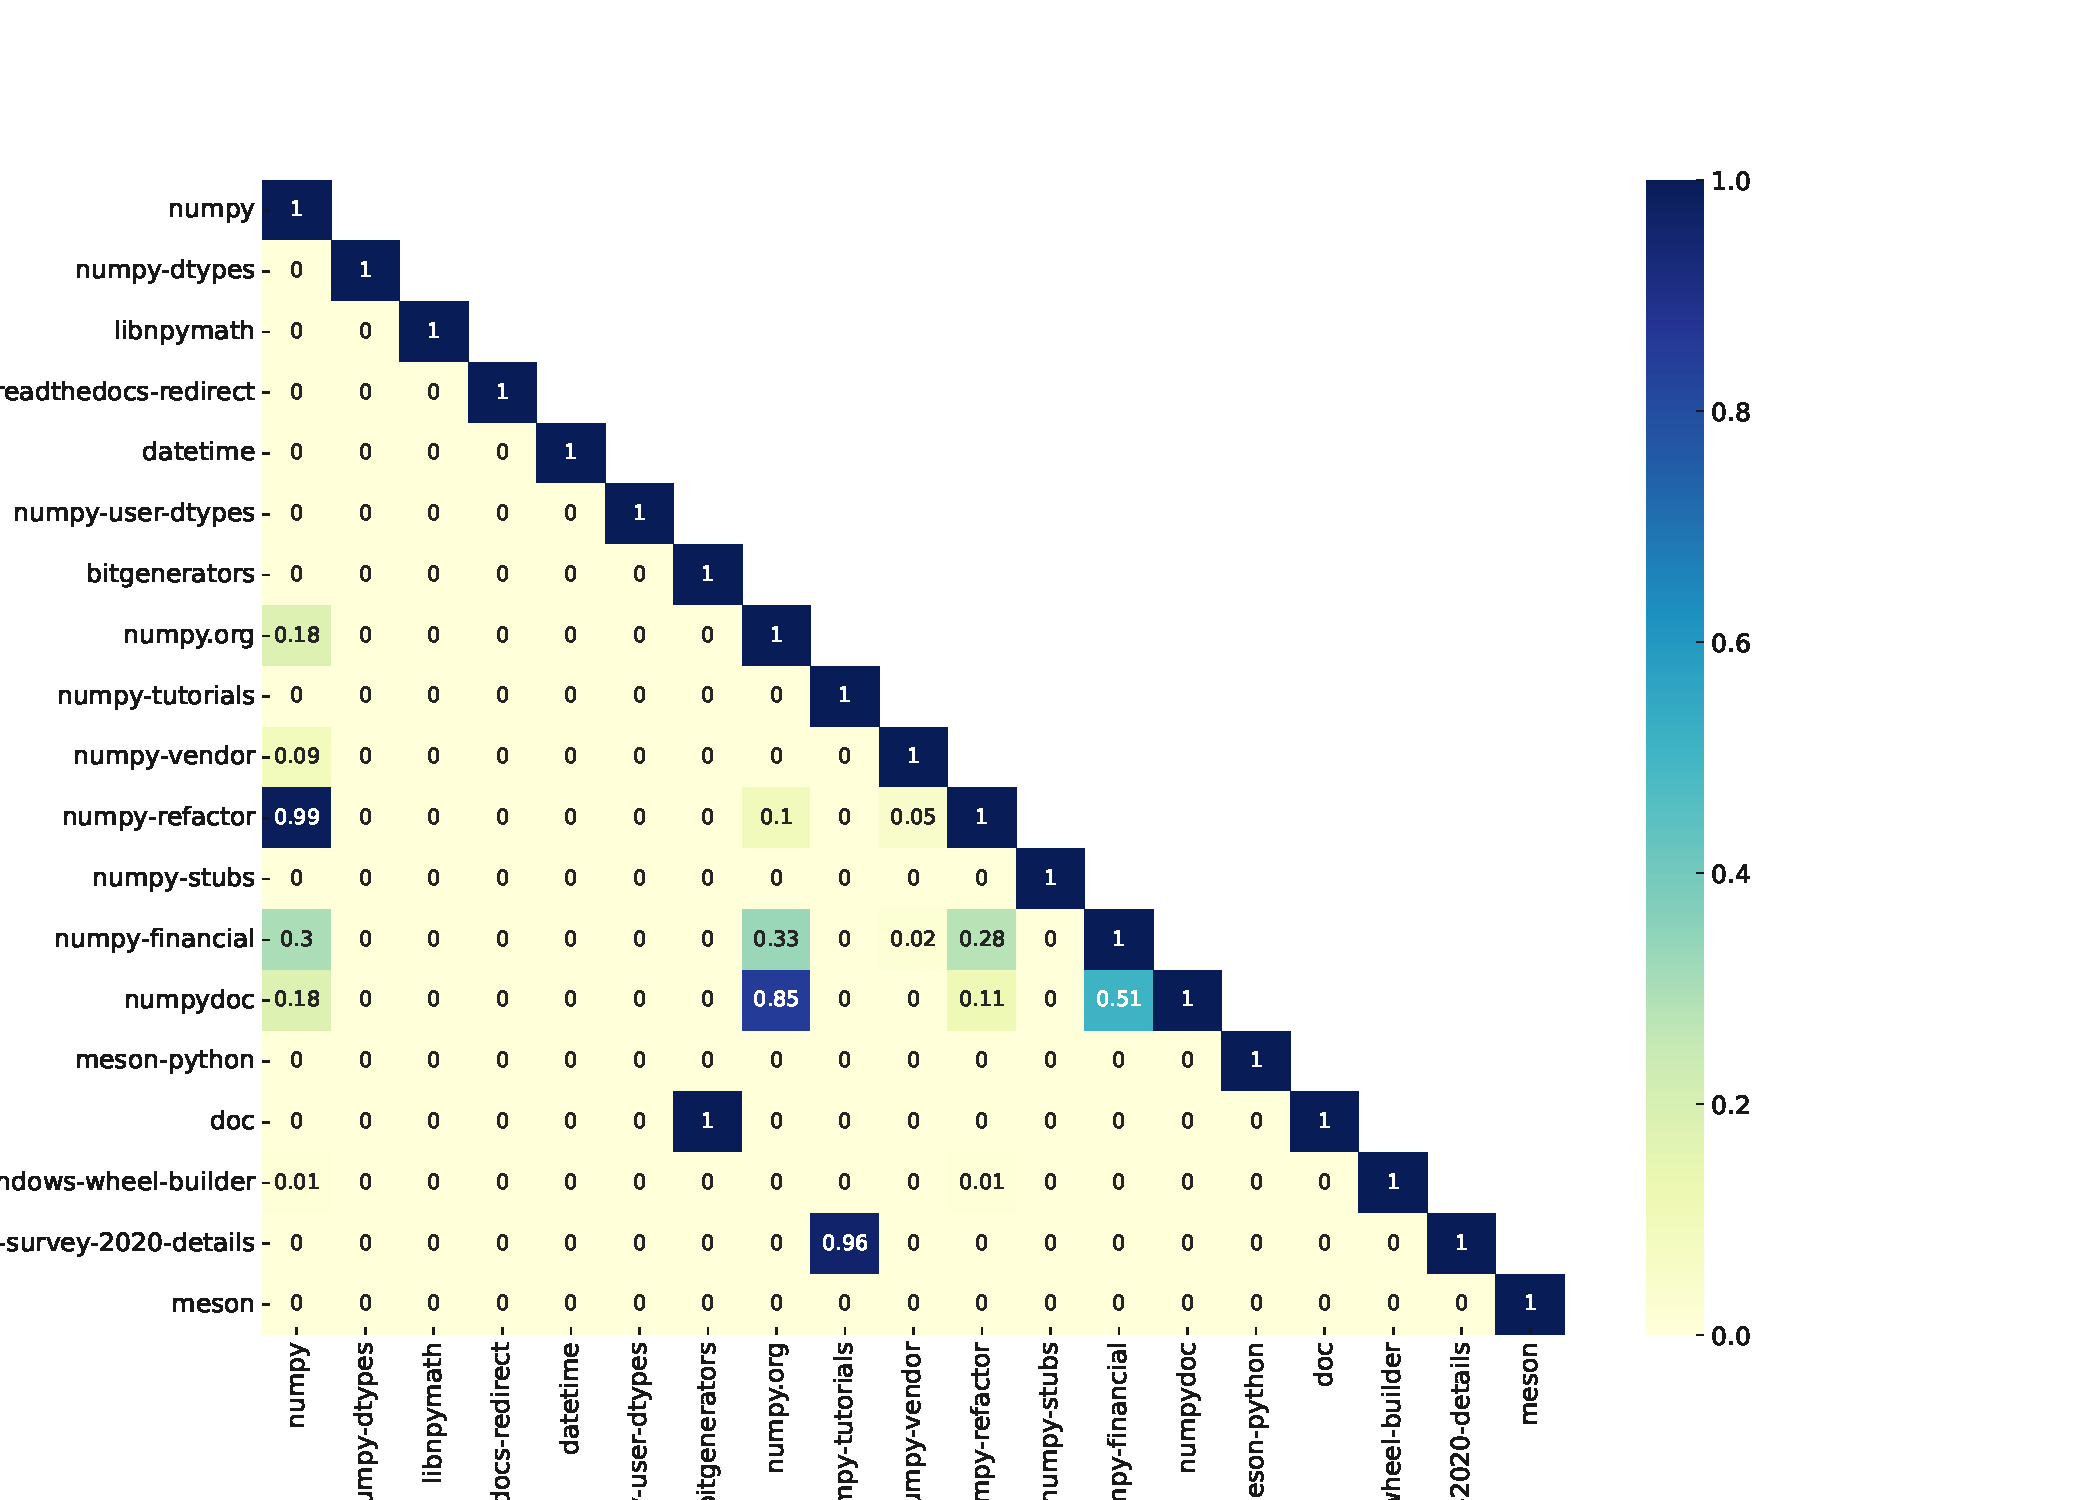
\includegraphics[width=\columnwidth]{Noguchi_fig/dev_cosine_sim_matrix_heatmap.pdf}
        \caption{NumPyにおける開発者のコサイン類似度}
        \label{fig:dev_similarity}
    \end{minipage}
    \begin{minipage}{1.0\columnwidth}
        \centering
        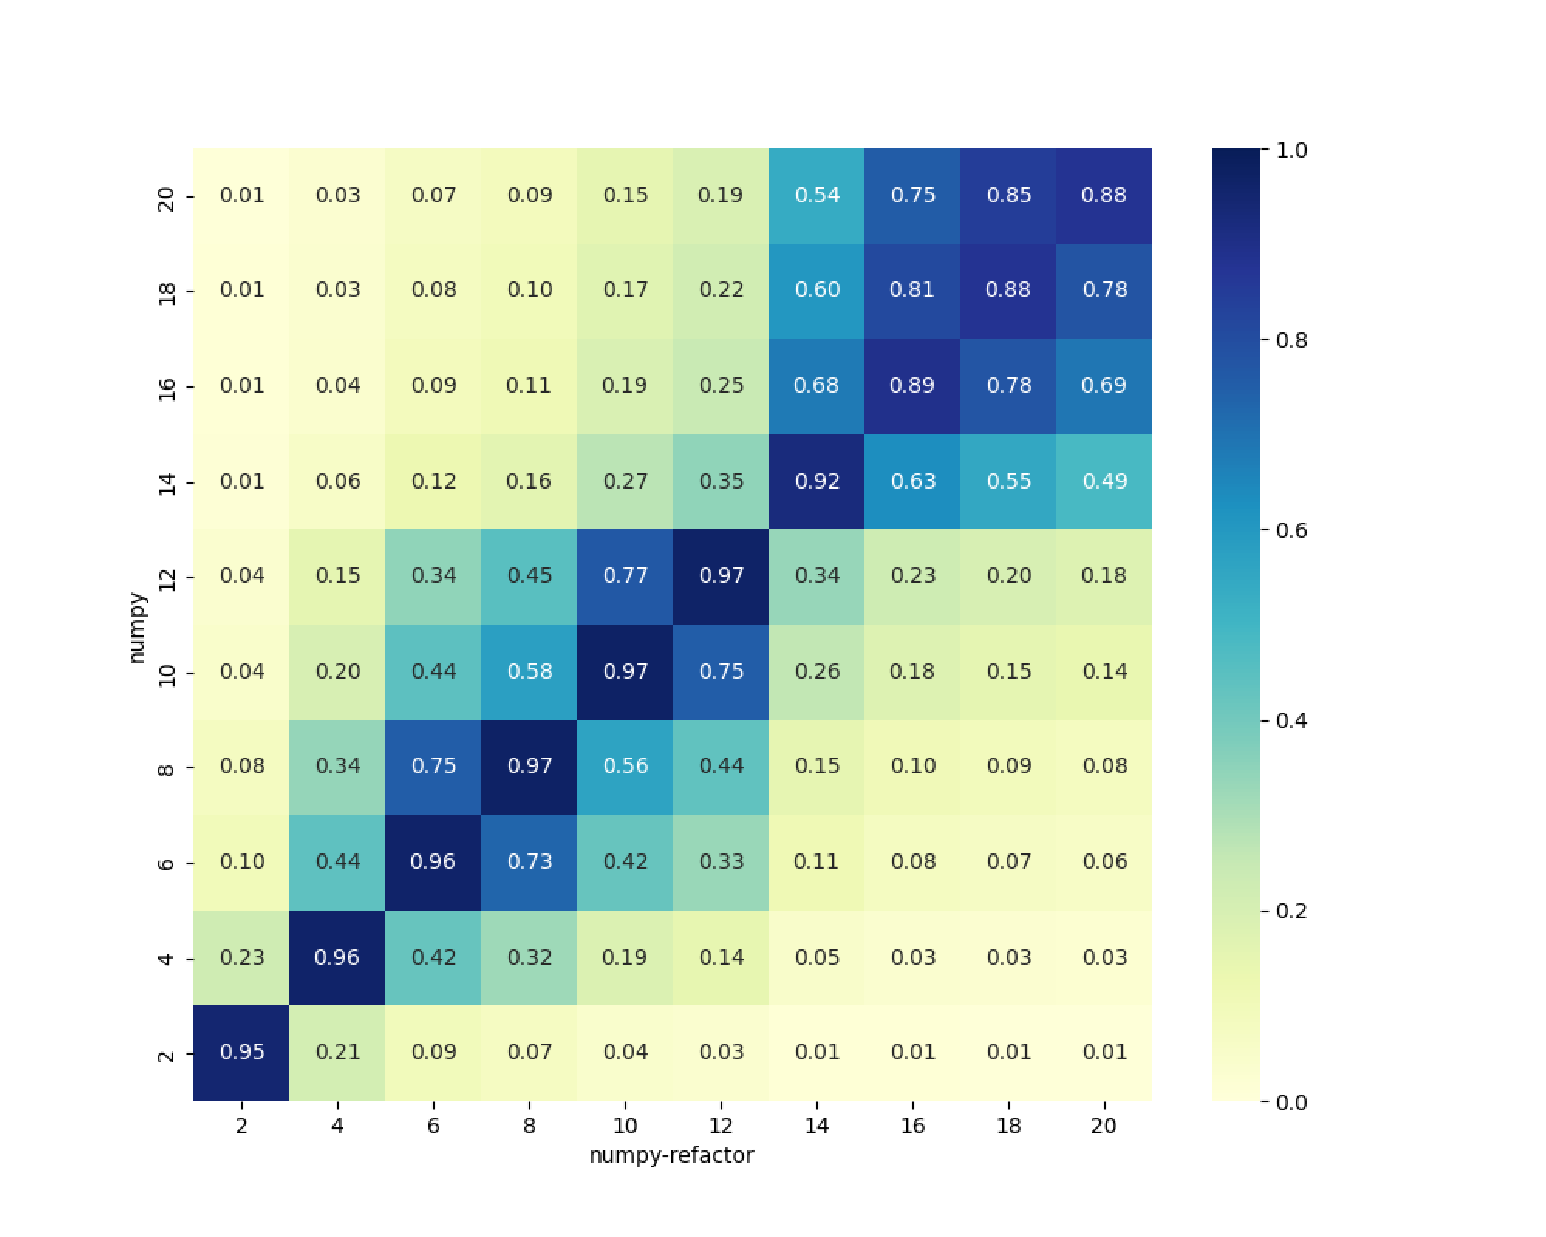
\includegraphics[width=\columnwidth]{Noguchi_fig/num_numref.pdf}
        \caption{numpy, numpy-refactorにおけるパターンの一致度}
        \label{fig:num_numref_match}
    \end{minipage}
\end{figure*}


次に,開発者の類似度が高いnumpyとnumpy-refactorで\ref{subsubsec:collect_pattern}章の手法を用いて収集されたパターンの信頼度を調査する.

分析対象としたnumpyとnumpy-refactorにて生成されたパターンを\ref{subsubsec:filtering}章の手法を用いて単体で信頼度を計測した結果が表\ref{table:single}である.
% RQ1において,分析対象とした3つの組み合わせについて分析を行う.numpy,numpy-refactor,numpy-financial,numpydocの4つのプロジェクト単体で,\ref{subsubsec:filtering}章の手法を用いて,パターンの信頼度を図る.次にRQ1で分析した3つのプロジェクトの組み合わせにおいて作成されたパターンを統合し,パターンの信頼度を図る.この時,RQ1で一致率が最も高い組み合わせのサポート値でフィルタリングした後のパターンを用いる.

それぞれの単体でパターンの信頼度を測定した結果が表\ref{table:single},パターンを統合して信頼度を測定した結果が\todo{\ref{table:merge}}である.
結果としては,numpy-refactorでは,numpyをパターンの増強に使用することで,信頼度が10\%以上のパターンが31件増加した.

\begin{table*}[t]
\centering
\caption{単体で作成されたパターンを元にテストデータでパターンの信頼度を測定した結果}
\label{table:single}
\begin{tabular}{l|rr}
\hline\hline
対象            & \multicolumn{1}{l}{元パターン数} & \multicolumn{1}{l}{フィルタリング後パターン数} \\ \hline
numpy           & 79,109                             & 3                                     \\ 
numpy-refactor  & 74,879                             & 7                                     \\ \hline
\end{tabular}
\end{table*}


% \begin{table*}[t]
% \caption{2つのプロジェクトで作成されたパターンを元にパターンの信頼度を測定した結果}
% \label{table:merge}
% \centering
% \begin{tabular}{l|lrrrr}\hline\hline
% 対象              & 統合先             & \multicolumn{1}{l}{パターン数(前)} & \multicolumn{1}{l}{パターン数(信頼度10\%以上)} & \multicolumn{1}{l}{中央値} & \multicolumn{1}{l}{平均値} \\ \hline
% numpy           & numpy-refactor  & 153,988                             & 3                                    & 1.0                     & 0.89                    \\
% numpy-refactor  & numpy           & 153,988                             & 38                                   & 1.0                     & 0.96                    \\ \hline
\begin{table*}[t]
\begin{tabular}{l|l|l|r|ll}
\hline\hline
対象 & 統合先 & パターン数 & \multicolumn{1}{l|}{サポート値} & 変更前 & 変更後 \\ \hline
numpy & \begin{tabular}[c]{@{}l@{}}numpy\\ -refactor\end{tabular} & \multicolumn{1}{r|}{3} & 5 & NAME=NUMBER & NAME=NUMBER \\
 &  &  & 4 & NAME=NONE & NAME=`c' \\
 &  &  & 3 & open & file \\ \hline
\begin{tabular}[c]{@{}l@{}}numpy-\\ refactor\end{tabular} & numpy & \multicolumn{1}{r|}{38} & 33 & TD(P,NAME=STRING) & TD(M,NAME=STRING) \\
 &  &  & 7 & NAME=NAME.strip(NAME) & NAME=string.strip(NAME) \\
 &  &  & 6 & \begin{tabular}[c]{@{}l@{}}NAME=NAME\_find\_common\_type\\ ({[}STRING, STRING`i2'{]}, {[}STRING{]})\end{tabular} & \begin{tabular}[c]{@{}l@{}}NAME=NAME\_find\_common\_type\\ ({[}STRING, STRING`i4'{]}, {[}STRING{]})\end{tabular} \\ \hline
\end{tabular}
\end{table*}
% \begin{table*}[t]
% \centering
% \begin{tabular}{l|l|l|l|r}
% \hline\hline
% 対象             & 統合先            & パターン数                   & パターン例                                                                                                                & \multicolumn{1}{l}{サポート値} \\ \hline
% numpy          & \begin{tabular}[c]{@{}l@{}}numpy\\ -refactor\end{tabular} & \multicolumn{1}{r|}{3}  & \colorbox{lightgray}{\texttt{NAME=}} \colorbox{lightgray}{\texttt{- NUMBER}} \colorbox{lightgray}{\texttt{+ NUMBER}}                                                                                                & 5                         \\ \cline{4-5} 
%                &                &                         & \colorbox{lightgray}{\texttt{NAME=}} \colorbox{lightgray}{\texttt{- None}} \colorbox{lightgray}{\texttt{+ 'c'}}                                                                                                       & 4                         \\ \cline{4-5} 
%                &                &                         & \colorbox{lightgray}{\texttt{- open}} \colorbox{lightgray}{\texttt{+ file}}                                                                                                          & 3                         \\ \hline
% \begin{tabular}[c]{@{}l@{}}numpy\\ -refactor\end{tabular} & numpy          & \multicolumn{1}{r|}{38} & \colorbox{lightgray}{\texttt{TD(}} \colorbox{lightgray}{\texttt{- P}} \colorbox{lightgray}{\texttt{+ M}} \colorbox{lightgray}{\texttt{,NAME=STRING}}),                                                                                                & 33                        \\ \cline{4-5} 
%                &                &                         & \colorbox{lightgray}{\texttt{NAME=}} \colorbox{lightgray}{\texttt{- NAME}} \colorbox{lightgray}{\texttt{+ string}} \colorbox{lightgray}{\texttt{.strip(}} \colorbox{lightgray}{\texttt{+ NAME}} \colorbox{lightgray}{\texttt{)}}                                                                                       & 7                         \\ \cline{4-5} 
%                &                &                         & \begin{tabular}[c]{@{}l@{}}\colorbox{lightgray}{\texttt{NAME=NAME.find\_common\_type({[}STRING,STRING,}} \\ \colorbox{lightgray}{\texttt{- 'i2'}} \colorbox{lightgray}{\texttt{+ 'i4'}} \colorbox{lightgray}{\texttt{],[STRING]}})\end{tabular} & 6                         \\ \hline
% \end{tabular}
% \caption{パターン例とサポート値}
% \label{table:pattern_example}
% \end{table*}

%%%%%%%%%%%%%%%%%%%%%%%%%%%
%5章考察
\section{考察}\label{sec:discussion}
%%%%%%%%%%%%%%%%%%%%%%%%%%%
\ref{sec:casestudy}章では,開発者と

%%%%%%%%%%%%%%%%%%%%%%%%%%%
%6章終わりに
\section{終わりに}\label{sec:conclusion}
%%%%%%%%%%%%%%%%%%%%%%%%%%%

%================
%\section*{参考文献}
%================
\bibliographystyle{junsrt}
\bibliography{NoguchiFOSE}

\end{document}
